\begin{figure}[H] 
\centering 
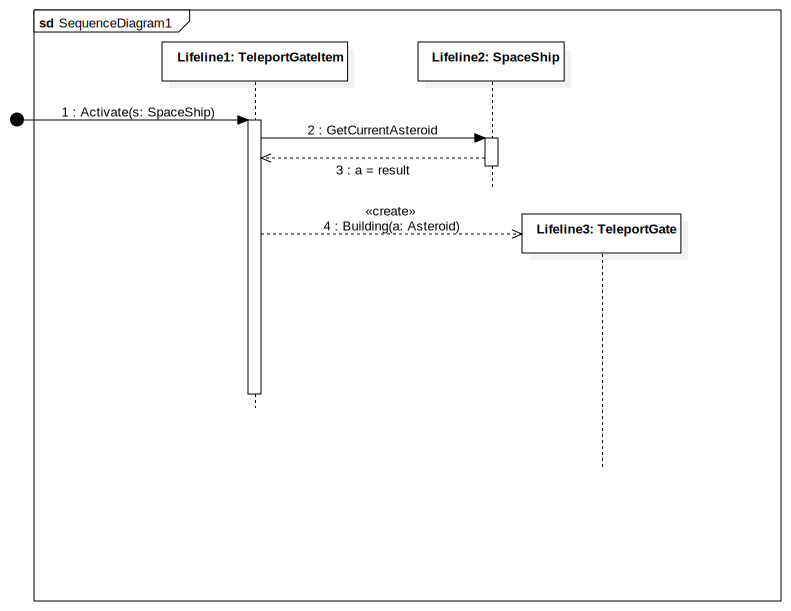
\includegraphics[width=1\textwidth]{docs/img/svg/Skeleton!Place gate!Interaction1!SequenceDiagram1_34.png} 
\caption{Test docs
} 
\end{figure} 

\begin{figure}[H] 
\centering 
\includegraphics[width=1\textwidth]{docs/img/svg/Skeleton!Solar flare!Interaction1!Tester queues solar flare for nex round_34.png} 
\caption{A tesztelő be tudja állítani, hogy a kör végén legyen-e napkitörés.} 
\end{figure} 

\begin{figure}[H] 
\centering 
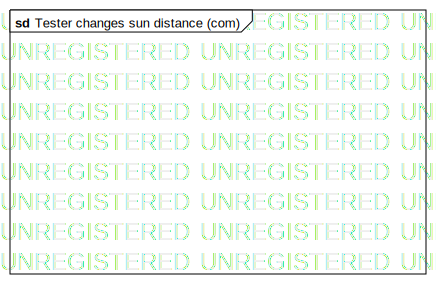
\includegraphics[width=1\textwidth]{docs/img/svg/Skeleton!Move asteroid field!Change Sun Distance!Communication!Tester changes sun distance (com)_37.png} 
\end{figure} 

\begin{figure}[H] 
\centering 
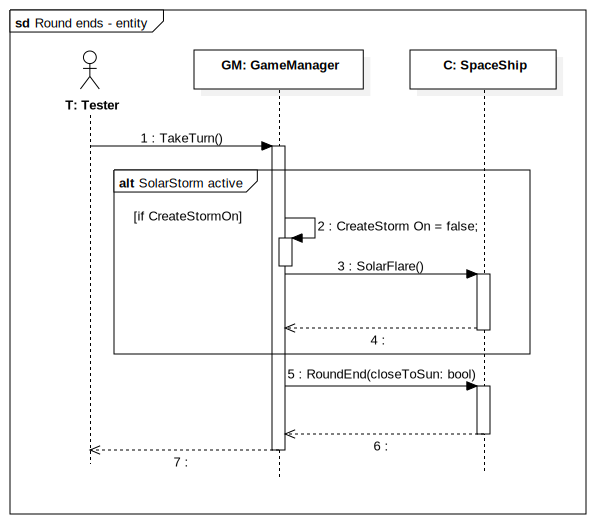
\includegraphics[width=1\textwidth]{docs/img/svg/Skeleton!Move asteroid field!Collaboration2!Sequence!Round ends - entity_39.png} 
\caption{Az űrjárműveken leken is meghívódik a RoundEnd függvény. Őket nem befolyásolja a napközelség.
Az aszteroidákat azonban igen, ők külön ábrázolva vannak!} 
\end{figure} 

